% Nallino, Part II p. 243, first figure: Mercury's deferent and equant, redrawn from the print at the size of the
% print. The coordinates are those of a 400 dpi render of the figure (crop from x 330 pt, y 222 pt of the master
% page; y downward). The upper circle has its centre in M, the lower in E'; the small circle (the circellus) has its
% centre in F (marked with a dot), M and E' on it; E (marked with a dot) is the Earth. A stray mark to the right of
% the circles is not drawn.
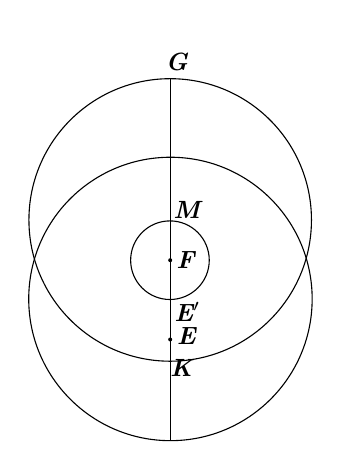
\begin{tikzpicture}[x=0.0635mm,y=-0.0635mm,line width=0.4pt,every node/.style={font=\bfseries\itshape\small,inner sep=1pt}]
\path (260,3.5);
\draw (545,388) circle[radius=282.5];
\draw (545.5,546) circle[radius=283.4];
\draw (544.5,468.5) circle[radius=78.6];
\draw (545,105) -- (545,830);
\fill (545,468.5) circle[radius=4];
\fill (545,627) circle[radius=4];
\node at (558,72) {G};
\node at (578,369) {M};
\node at (575.5,467.5) {F};
\node at (572,572) {E\rlap{$'$}};
\node at (577,619) {E};
\node at (567,684) {K};
\end{tikzpicture}
